\documentclass{standalone}
\usepackage{tikz}
\begin{document}
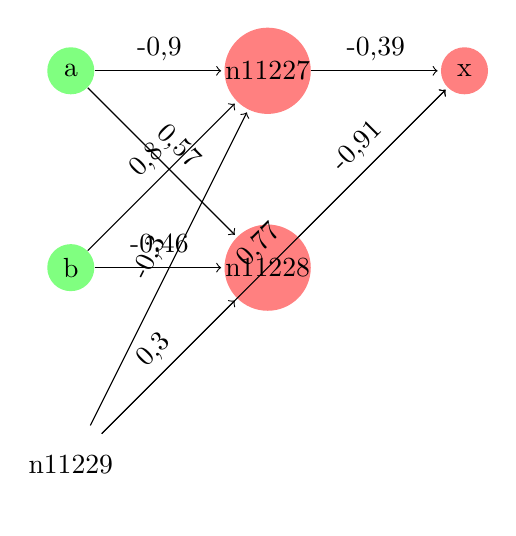
\begin{tikzpicture}[shorten >=1pt,->,draw=black!,node distance=2.5cm]
\tikzstyle{neuron}=[circle,fill=black!25,minimum size=17pt,inner sep=0pt]
\tikzstyle{constant}=[neuron, fill=white!50];
\tikzstyle{sigmoid}=[neuron, fill=red!50];
\tikzstyle{identity}=[neuron, fill=green!50];
\node [identity] (a) {a};
\node [identity,below of=a] (b) {b};
\node [constant,below of=b] (n11229) {n11229};
\node [sigmoid,right of=a] (n11227) {n11227};
\node [sigmoid,below of=n11227] (n11228) {n11228};
\node [sigmoid,right of=n11227] (x) {x};
\path[every node/.style={sloped,anchor=south,auto=false}]
(n11229) edge node {0,77} (x)
(n11229) edge node {-0,3} (n11227)
(n11229) edge node {0,3} (n11228)
(n11227) edge node {-0,39} (x)
(n11228) edge node {-0,91} (x)
(a) edge node {0,57} (n11228)
(a) edge node {-0,9} (n11227)
(b) edge node {0,8} (n11227)
(b) edge node {-0,46} (n11228)
;\end{tikzpicture}
\end{document}